\documentclass[]{book}

%These tell TeX which packages to use.
\usepackage{array,epsfig}
\usepackage{amsmath}
\usepackage{amsfonts}
\usepackage{amssymb}
\usepackage{amsxtra}
\usepackage{amsthm}
\usepackage{mathrsfs}
\usepackage{color}
\usepackage{tikz}
\usepackage{enumerate}
\usepackage{hyperref}


%Here I define some theorem styles and shortcut commands for symbols I use often
\theoremstyle{definition}
\newtheorem{defn}{Definition}
\newtheorem{thm}{Theorem}
\newtheorem{cor}{Corollary}
\newtheorem*{rmk}{Remark}
\newtheorem{lem}{Lemma}
\newtheorem*{joke}{Joke}
\newtheorem{ex}{Example}
\newtheorem*{soln}{Solution}
\newtheorem{prop}{Proposition}

\newcommand{\lra}{\longrightarrow}
\newcommand{\ra}{\rightarrow}
\newcommand{\surj}{\twoheadrightarrow}
\newcommand{\graph}{\mathrm{graph}}
\newcommand{\bb}[1]{\mathbb{#1}}
\newcommand{\Z}{\bb{Z}}
\newcommand{\Q}{\bb{Q}}
\newcommand{\R}{\bb{R}}
\newcommand{\C}{\bb{C}}
\newcommand{\N}{\bb{N}}
\newcommand{\M}{\mathbf{M}}
\newcommand{\m}{\mathbf{m}}
\newcommand{\MM}{\mathscr{M}}
\newcommand{\HH}{\mathscr{H}}
\newcommand{\Om}{\Omega}
\newcommand{\Ho}{\in\HH(\Om)}
\newcommand{\bd}{\partial}
\newcommand{\del}{\partial}
\newcommand{\bardel}{\overline\partial}
\newcommand{\textdf}[1]{\textbf{\textsf{#1}}\index{#1}}
\newcommand{\img}{\mathrm{img}}
\newcommand{\ip}[2]{\left\langle{#1},{#2}\right\rangle}
\newcommand{\inter}[1]{\mathrm{int}{#1}}
\newcommand{\exter}[1]{\mathrm{ext}{#1}}
\newcommand{\cl}[1]{\mathrm{cl}{#1}}
\newcommand{\ds}{\displaystyle}
\newcommand{\vol}{\mathrm{vol}}
\newcommand{\cnt}{\mathrm{ct}}
\newcommand{\osc}{\mathrm{osc}}
\newcommand{\LL}{\mathbf{L}}
\newcommand{\UU}{\mathbf{U}}
\newcommand{\support}{\mathrm{support}}
\newcommand{\AND}{\;\wedge\;}
\newcommand{\OR}{\;\vee\;}
\newcommand{\Oset}{\varnothing}
\newcommand{\st}{\ni}
\newcommand{\wh}{\widehat}

%Pagination stuff.
\setlength{\topmargin}{-.3 in}
\setlength{\oddsidemargin}{0in}
\setlength{\evensidemargin}{0in}
\setlength{\textheight}{9.in}
\setlength{\textwidth}{6.5in}
\pagestyle{empty}



\begin{document}


\begin{center}
{\Large Machine learning \hspace{0.5cm} ex-ch2 1}\\
\textbf{Understanding Machine Learning: From Theory to Algorithms [Exercise 2.4]}\\
\textbf{Mehrnaz jalili}\\ %You should put your name here
\textit{Email: \href{mailto:Mehrnazjalili1991@gmail.com}{Mehrnazjalili1991@gmail.com}} 

Date: \today %You should write the date here.
\end{center}

\vspace{0.2 cm}


\subsection*{Exercises for Section 2.4.1: Overfitting of polynomial matching}
We have shown that the predictor defined in Equation (2.3) leads to overfitting. While this predictor seems to be very unnatural,the goal of this exercise is to show that it can be described as a thresholded polynomial. That is, show that given a training set $S=\{(x_i,f(x_i))\}^m_{i=1}\subseteq (\mathbb{R}^d\times \{0,1\})^m$, there exists a polynomial $p_S$ such that $h_S(x)=1$ if and only if $p_S(x)\geq 0$, where $h_S$ is as defined in Equation (2.3). It follows that learning the class of all thresholded polynomials using the ERM rule may lead to overfitting.

\vspace{0.5cm}

First, we define the concept of "Norm": Given a vector space $\displaystyle X$ over a subfield $F$ of the complex numbers $\mathbb C$ , a \textbf{Norm} on $\displaystyle X$ is a real-valued function $\displaystyle \left\| * \right\|:X\to \mathbb R $ with the following properties, where $\displaystyle |s|$ denotes the usual absolute value of a scalar $\displaystyle s$:

\begin{enumerate}
    \item Subadditivity/Triangle inequality: ${\displaystyle \left\|x+y\right\| \leq \left\|x\right\|+\left\|y\right\|}$ for all ${\displaystyle x,y\in X}$.
    \item Absolute homogeneity: ${\displaystyle \left\|sx\right\|=\left|s\right|.\left\|x\right\|}$ for all $x\in X$ and and all scalars $s$. 
    \item Positive definiteness/Point-separating: for all ${\displaystyle x\in X}$, if $\left\|x\right\|=0$ then $x=0$.
    \item Nonnegativity: $\left\| x \right\| \geq 0$ for all $x\in X$
\end{enumerate}
Consider an arbitrary norm so that $\left\| * \right\|:\mathbb{R}^d\rightarrow \mathbb{R} $. We are looking for a polynomial function which returns a negative value whenever $h_S(x)=1$. A simple solution to this problem is setting the function's value to $0$ at points  whenever $h_S(x)=1$. we achieved this by multiplying $\left \| x-x_j \right \|$s such that $j \in J$ (It is noteworthy that $J=\{j\in [m]:h_S(x_j)=1 \}$) \footnote{m is the cardinal of our training set} But we have two main problems. First, the value of the function must be negative at the points $h_s(x)=0$, which can be reached by multiplying the expression by a $(-1)$. The second problem is that its function will change the sign at the points $x_j$. So we consider each element to the power of an arbitrary positive number such as 4.

\begin{equation*}
    p_S(x)=-\prod_{j\in J}\left \| x-x_j \right \|^4
\end{equation*}

Now we can see that $p_S(x)=0$ (or with a deeper look $p_S(x)\geq 0$) if and only if $h_S(x)=1$

\subsection*{Exercises for Section 2.4.2}
Let $\mathcal{H}$ be a class of binary classifiers over a domain $\mathcal{X}$ . Let $\mathcal{D}$ be an unknown distribution over $\mathcal{X}$ , and let f be the target hypothesis in $\mathcal{H}$.
Fix some $h \in \mathcal{H}$. Show that
the expected value of $L_S(h)$ over the choice of $S|_x$ equals $L_{(\mathcal{D},f)}(h)$, namely,
\begin{equation*}
   \underset{S|_x \sim \mathcal{D}^m}{\mathbb{E}}[L_S(h)]=L_{(\mathcal{D},f)}(h)
\end{equation*}
  
  \vspace{0.5cm}
  
  First, let's take a closer look at the definitions and theorems. We have defined the error of a prediction rule, $h:\mathcal{X} \rightarrow  \mathcal{Y}$, to be
  \begin{equation*}
      L_{\mathcal{D},f}(h) \overset{\textup{def}}{=}  \underset{x \sim \mathcal{D}}{\mathbb{P}}[h(x)\neq f(x)] \overset{\textup{def}}{=} \mathcal{D}(\{x:h(x) \neq f(x)\})\overset{\textup{def}}{=}\mathbb{E}_{x \sim \mathcal{D}}[1_{h(x)\neq f(X)}]
  \end{equation*}
  
  In addition, we have proved by the right most expression of the above equalities that $L_{\mathcal{D},f}(h)=\mathbb{E}[L_S(h)]$.
  Inspired by the aforementioned proof, we will try to start with $\mathbb{E}_{x \sim \mathcal{D}}[1_{h(x)\neq f(X)}]$ and complete the proof by expanding expressions.
  Before we start proving, we define the set $J$ to be $J=\{j\in [m] ,1\leq j \leq |S|\}$.\footnote{S is our training set and $|S|=m$}
  %\mathbb{E}_{x \sim \mathcal{D}}[1_{h(x)\neq f(X)}]
  
  
   \textbf{The first method:}
  
  \begin{align*}
      \underset{S|_x \sim \mathcal{D}^m}{\mathbb{E}}[L_S(h)] & =\underset{S|_x \sim \mathcal{D}^m}{\mathbb{E}}\left [\frac{1}{m}\sum_{j\in J}[1_{h(x_j)\neq f(x_j)}]\right ] \\
     & =\frac{1}{m}\sum_{j\in J} \left ( \underset{x_j \sim \mathcal{D}}{\mathbb{E}}\left [1_{h(x_j)\neq f(x_j)}\right ] \right ) && \text{(by linearity)}
     \\
     & =\frac{1}{m}\sum_{j\in J} \left ( \underset{x \sim \mathcal{D}}{\mathbb{E}}\left [1_{h(x)\neq f(x)}\right ] \right ) && \text{(by i.i.d)}
      \\
     & =\frac{1}{m} \times m \times \left ( \underset{x \sim \mathcal{D}}{\mathbb{E}}\left [1_{h(x)\neq f(x)}\right ] \right ) && \text{(Since the $|J|=m$)}
     \\
     &= L_{\mathcal{D},f}(h) && \text{generalization error}
  \end{align*}
  
     \textbf{The second method:}
     
       \begin{align*}
      \underset{S|_x \sim \mathcal{D}^m}{\mathbb{E}}[L_S(h)] & =\underset{S|_x \sim \mathcal{D}^m}{\mathbb{E}}\left [\frac{1}{m}\sum_{j\in J}[1_{h(x_j)\neq f(x_j)}]\right ] \\
     & =\frac{1}{m}\sum_{j\in J} \left ( \underset{x_j \sim \mathcal{D}}{\mathbb{E}}\left [1_{h(x_j)\neq f(x_j)}\right ] \right ) && \text{(by linearity)}
     \\
     & =\frac{1}{m}\sum_{j\in J} \left ( \underset{x_j \sim \mathcal{D}}{\mathbb{P}}\left [{h(x_j)\neq f(x_j)}\right ] \right ) 
     \\
      & =\frac{1}{m}\sum_{j\in J} \left ( \underset{x \sim \mathcal{D}}{\mathbb{P}}\left [{h(x)\neq f(x)}\right ] \right ) && \text{(by i.i.d)}
      \\
     & =\frac{1}{m} \times m \times  L_{\mathcal{D},f}(h) && \text{(by the definition of $L_{\mathcal{D},f}(h)$ )} 
     \\
     &= L_{\mathcal{D},f}(h) && \text{generalization error}
  \end{align*}
    
\subsection*{Exercises for Section 2.4.3: Axis aligned rectangles}

An axis aligned rectangle classifier in the plane is a classifier that assigns the value $1$ to a point if and only if it is inside a certain rectangle.
Formally, given real numbers $a_1 \leq b_1, \hspace{0.2 cm} a_2 \leq b_2 $, define the classifier $h_{(a_1.b_1,a_2,b_2)}$ by

\begin{equation*}
   h_{(a_1.b_1,a_2,b_2)}(x_1,x_2)= \left\{\begin{matrix}
1 &  \text{if} \hspace{0.1cm} a_1 \leq x \leq b_1 \hspace{0.2cm} \text{and} \hspace{0.2cm} a_2 \leq x_2 \leq b_2 \\ 
0 & \text{otherwise}
\end{matrix}\right. 
\end{equation*}

The class of all axis aligned rectangles in the plane is defined as

\begin{equation*}
    \mathcal{H}_{\text{rec}}^2=\{ h_{(a_1.b_1,a_2,b_2)}:a_1 \leq b_1 \hspace{0.1 cm}, \text{and}\hspace{0,1 cm} a_2\leq b_2\}
\end{equation*}

Note that this is an infinite size hypothesis class. Throughout this exercise we rely
on the realizability assumption.

\begin{enumerate}
    \item Let A be the algorithm that returns the smallest rectangle enclosing all positive
examples in the training set. Show that A is an \textbf{ERM}.
\item Show that if A receives a training set of size $\geq \frac{4 \log (\frac{4}{\delta}) }{\epsilon}$ then, with probability of at least $1-\delta$ it returns a hypothesis with error of at most $\epsilon$ .

\textit{Hint}: Fix some distribution $\mathcal{D}$ over $\mathcal{X}$, let $R^*=R(a_1^*,b_1^*,a_2^*,b_2^*)$ be the rectangle that generates the labels, and let $f$ be the corresponding hypothesis. Let $a_1 \geq a_1^*$ be a number such that the probability mass (with respect to $\mathcal{D}$) of the rectangle $R_1=R(a_1^*,a_1,a_2^*,b_2^*)$ is exactly $\frac{\epsilon}{4}$. Similarly, let $b_1,a_2,b_2$ be numbers such that the probability masses of the rectangles $R_2=R(b_1,b_1^*,a_2^*,b_2^*)$, $R_3=R(a_1^*,b_1^*,a_2^*,a_2)$, $R_4=R(a_1^*,b_1^*,b_2,b_2^*)$ are all exactly $\frac{\epsilon}{4}$. Let $R(s)$ be the rectangle returned by A. See illustration in Figure 2.2.
\begin{itemize}
    \item Show that $R(S)\subseteq R^*$.
    \item Show that if $S$ contains (positive) examples in all of the rectangles $R_1$, $R_2$, $R_3$, $R_4$, then the hypothesis returned by $A$ has error of at most $\epsilon$.
    \item For each $i\in \{1,...,4\}$, upper bound the probability that $S$ does not contain an example from $R_i$ .
    \item Use the union bound to conclude the argument.
\end{itemize}
\item Repeat the previous question for the class of axis aligned rectangles in $\mathbb{R}^d$.
\item Show that the runtime of applying the algorithm $A$ mentioned earlier is polynomial in $d$, $\frac{1}{\epsilon}$, and in $\log \left ( \frac{1}{\delta} \right )$.
\end{enumerate}


\begin{center}

\tikzset{every picture/.style={line width=0.75pt}} %set default line width to 0.75pt        

\begin{tikzpicture}[x=0.75pt,y=0.75pt,yscale=-0.75,xscale=0.75]
%uncomment if require: \path (0,300); %set diagram left start at 0, and has height of 300

%Shape: Rectangle [id:dp10339158537804893] 
\draw  [line width=0.75]  (239.14,40.57) -- (460.86,40.57) -- (460.86,262.29) -- (239.14,262.29) -- cycle ;
%Shape: Rectangle [id:dp23259535297012635] 
\draw  [line width=0.75]  (211.43,12.86) -- (488.57,12.86) -- (488.57,290) -- (211.43,290) -- cycle ;
%Straight Lines [id:da25307621382117107] 
\draw [line width=0.75]    (156,151.43) -- (544,151.43) ;
%Shape: Rectangle [id:dp8527626214142721] 
\draw  [dash pattern={on 5.63pt off 4.5pt}][line width=1.5]  (211.43,12.86) -- (266.86,12.86) -- (266.86,290) -- (211.43,290) -- cycle ;

% Text Node
\draw (378.67,98.33) node [anchor=north west][inner sep=0.75pt]   [align=left] {+};
% Text Node
\draw (308.67,177.67) node [anchor=north west][inner sep=0.75pt]   [align=left] {+};
% Text Node
\draw (422,252.67) node [anchor=north west][inner sep=0.75pt]   [align=left] {+};
% Text Node
\draw (231,75.67) node [anchor=north west][inner sep=0.75pt]   [align=left] {+};
% Text Node
\draw (186.67,63) node [anchor=north west][inner sep=0.75pt]   [align=left] {\mbox{-}};
% Text Node
\draw (506.67,125) node [anchor=north west][inner sep=0.75pt]   [align=left] {\mbox{-}};
% Text Node
\draw (463.33,13.73) node [anchor=north west][inner sep=0.75pt]    {$R^{*}$};
% Text Node
\draw (415.67,51.4) node [anchor=north west][inner sep=0.75pt]    {$R( S)$};
% Text Node
\draw (450,32.33) node [anchor=north west][inner sep=0.75pt]   [align=left] {+};
% Text Node
\draw (238,268.07) node [anchor=north west][inner sep=0.75pt]    {$R_{1}$};


\end{tikzpicture}

\textbf{Figure 2.2}. Axis aligned rectangles.
    
\end{center}


\vspace{0.5cm}

\begin{enumerate}
    \item We have a training set which is called $S$. We also consider Algorithm $A$ to return the smallest rectangle containing all the positives as the output. It is clear that $A$ is a member of $\mathcal{H}$. Because $\mathcal{H}$ is the set of all rectangles in the universe. Furthermore, considering the  realizability assumption, we have at least one member of $\mathcal{H}$ such that $ L_s (h) = 0 $ Given that the output of Algorithm $A$ contains all positive labels and is clearly due to being the tiniest one, it is not going to mislabel negative elements, so $ L_S (A) = 0 $, therefore, $A \in \arg \underset{h \in \mathcal{H}}{\min} L_s(h)$. So $A$ is an ERM.
    \item 
       First, we consider everything that was raised in the Hint section of the question as basic assumptions. From the definition of Algorithm $A$ , it can be easily concluded that $ R(s) \subseteq R^* $.
    \begin{equation*}
        L_{(\mathcal{D},f)}=\mathcal{D}(R^*-R(S))
    \end{equation*}
    Second, we fix some $\epsilon \in (0,1)$ and then consider $R_i$ as hint.\footnote{For each $i\in \{1,2,3,4\}$.} Then we define another family of sets $\mathcal{F}$.
    \begin{equation*}
        F_i=\{S|_x:S|_x \cap R_i = \varnothing \}
    \end{equation*}
    
    Then we calculate the probability that $L_{(\mathcal{D},f)}$ being greater than $\epsilon$.
    \begin{equation*}
        \mathcal{D}^m \left ( \left \{  S:   L_{(\mathcal{D},f)}(R(s))>\epsilon \right \} \right ) \leq \mathcal{D}^m \left ( \bigcup_{i=1}^{4} F_i \right ) \leq \sum_{i=1}^{4} \mathcal{D}^m \left ( F_i \right )
    \end{equation*}
    

    \begin{equation*}
        \mathcal{D}^m(F_i)=(1-\frac{\epsilon}{4})^m \leq e^{-m*\frac{\epsilon}{4}}
    \end{equation*}
    Therefore,
    \begin{equation*}
        gin{equation*}
        \mathcal{D}^m \left ( \left \{  S:   L_{(\mathcal{D},f)}(R(s))>\epsilon \right \} \right ) \leq 4.e^{-m.\frac{\epsilon}{4}}
    \end{equation*}
    
    
    
    
    
    
    
    
    \item Formally, given real numbers $a_1 \leq b_1, \hspace{0.2 cm} a_2 \leq b_2 \hspace{0.2 cm} ... \hspace{0.2 cm} a_d \leq b_d $, define the classifier $h_{(a_1.b_1,...,a_d,b_d)}$ by

\begin{equation*}
  h_{(a_1.b_1,...,a_d,b_d)}(x_1,...,x_d)= \left\{\begin{matrix}
0 & \exists i \in [d] , x_i \notin (a_i,b_i)  \\ 
1 & \text{otherwise}
\end{matrix}\right. 
\end{equation*}

The class of all axis aligned rectangles in the plane is defined as

\begin{equation*}
    \mathcal{H}_{\text{rec}}^d=\{ h_{(a_1.b_1,...,a_d,b_d)}:\forall i \in [d],a_i \leq b_i\}
\end{equation*}
    Note that this is an infinite size hypothesis class. Throughout this exercise we rely
on the realizability assumption.
 
 \begin{enumerate}[I]
  \item Let $A$ be the algorithm that returns the smallest d-dimensional cube
  \footnote{In geometry, a \textbf{hypercube} is an n-dimensional analogue of a square $(n = 2)$ and a cube $(n = 3)$. It is a closed, compact, convex figure whose $1$-skeleton consists of groups of opposite parallel line segments aligned in each of the space's dimensions, perpendicular to each other and of the same length. A unit hypercube's longest diagonal in n dimensions is equal to ${ {\sqrt {n}}.}$
  An \textbf{n-dimensional hypercube} is more commonly referred to as an \textbf{n-cube} or sometimes as an \textbf{n-dimensional cube}.
  }
 containing all the training set's positive elements. Show that $A$ is an ERM.
  
  
  \item Show that if A receives a training set of size $\geq \frac{2d \log (\frac{2d}{\delta}) }{\epsilon}$ then, with probability of at least $1-\delta$ it returns a hypothesis with error of at most $\epsilon$ .
  
\end{enumerate}

\end{enumerate}

\vspace{5cm}
\begin{center}
    This project was written in collaboration with Arash Sajjadi.
\end{center}



\end{document}


